\documentclass{winslabreport}
\usepackage{hyperref}
\reporttitle{A Naive Implementation of BlindBox: Deep Packet Inspection
over Encrypted Traffic}
\coursename{CENG781 Network Security}
\courseterm{2018-2019 Spring}
\reportpurpose{Term Project Report}
\authorname{Cansin Yildiz, Fatma Demirtas, Seyma Bodur}
\studentnumber{1449271, 1927961, 1854512}
\useremail{cansin.yildiz@metu.edu.tr, fatma.demirtas@metu.edu.tr, bodur.seyma@metu.edu.tr}
\program{Computer Engineering}

\AtBeginDocument{% the counter is defined later
  \counterwithout{lstlisting}{chapter}%
}
\makeatletter
\renewcommand{\l@lstlisting}[2]{%
  \@dottedtocline{1}{0em}{3em}{\lstlistingname\ #1}{#2}%
}
\makeatother

\begin{document}
\renewcommand{\lstlistingname}{Code}
\renewcommand\lstlistlistingname{List of Code}
\restoregeometry
\maketitle

\summary
As Hyper Text Transfer Protocol Secure (HTTPS) becomes the new normal for The World Wide Web (WWW), Deep Packet Inspection (DPI) of encrypted streams becomes crucial than ever. Sherry and her colleagues claim to introduce the first system that simulta- neously provides the functionality of middleboxes and the privacy of encryption: BlindBox [4]. This system performs the deep-packet inspection directly on the encrypted traffic which makes it practical for real-world applications that use long-lived HTTPS connections.

In this paper, we provide a naive implementation for one of the core protocols described in the original work by Sherry et al.: BlindBox, Protocol I: Basic Detection. Using the protocol, we are implementing a way for clients to detect malicious payloads over encrypted traffic.

\tableofcontents
\addcontentsline{toc}{section}{\lstlistlistingname}
\lstlistoflistings
\listoffigures
\body

\section{Introduction}

Deep Packet Inspection (DPI), which is the computer network filtering technique, controls the content of the traffic and traffic flow \cite{Deep}. DPI is used in several areas such that protection to security threats, lawful interception, parental filtering. There are different middlebox approaches to provide the functionality of DPI. However, all of the existing approaches have one fundamental problem: while providing security, they do not put emphasis on privacy. BlindBox \cite{Blindbox}, which is a middlebox presented in this report, provide both functionality of the DPI and privacy of the packets. If the BlindBox is used as middlebox, there is no need to decrypt the payload. Inspecting packets is made over encrypted payload. 

\section{Background and Related Work}

\subsection{Background}

There are many related works on middleboxes. Some of them are considered insecure. As explained in \cite{SSL}, man in the middle attack is built using counterfeit certificates on SSL by some systems. In that way, security of the SSL could be broken, and middlebox can decrypt the traffic for detection scan. That is, E2E security of SSL is destroyed which is insecure. In addition, there is a system called Meddle \cite{Traffic}. Its goal is to increase transparency in mobile networks. This is done by endpoints and the third-party are authorized to control the traffic, which is not required in BlindBox. The systems APLOMB \cite{Network} and Beyond the Radio \cite{48} are similar to Meddle.

Some middleboxes use encrypted payload for detection. But, they have some properties that are not required for BlindBox. For example,  fully homomorphic encryption\cite{24} and general functional encryption \cite{23} can be used in order to encrypt the payload. Their computation speed is so slow when they are compared with an encryption scheme used in BlindBox.

Also, searchable encryption schemes can be used in order to encrypt the rules. However, such schemes encrypt the rules in such a way that it does not meet the security which BlindBox require. In addition, symmetric key searchable scheme \cite{46} and public key encryption with searching  \cite{19} can also be used for packet processing. However, they have some weakness: symmetric key searchable scheme is slower than the scheme which BlindBox uses, and the public key searchable scheme is also not proper for performance because it should create cryptographic pairs for each token.

All these means, security and speed desires cannot be obtained by all these encryption schemes. Therefore, BlindBox uses different encryption scheme which is called DPIEnc. DPIEnc takes the speed of deterministic searchable encryption scheme and it takes the security of the randomized encryption scheme.   

\subsection{Related Work} 

BlindBox ensures the following properties:

\begin{itemize}
	\item It seeks for suspicious content for security. 
	\item Sender and receiver do not have an idea what the rules are.
	\item It must have at least one trusted endpoint as in intrusion detection (IDS). 
	\item It does not decrypt the actual payload, so the privacy is not compromised.
\end{itemize}

The last property is the main difference between BlindBox, other similar middleboxes that aim for DPI. \autoref{fig:bli1} outlines how BlindBox works.

\begin{figure}[H]
	\centering
	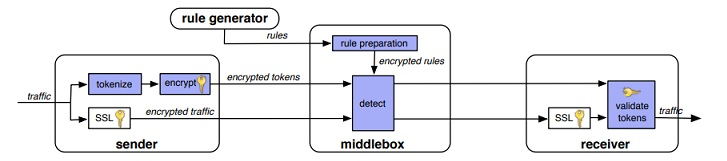
\includegraphics[width=150mm,height=35mm]{blindbox.jpg}
	\caption{BlindBox Architecture}
	\label{fig:bli1}
\end{figure}

There are three different keys to use in this scheme. First one is $k_{SSL}$ which is used in SSL protocol. The second one is k which is used for detection. The last one is $k_r$ and which is used for randomness. These three keys are generated/derived by $k_0$ which is the key sender and receiver agree by SSL Handshake. In that way, sender and receiver are connected.

As it is seen in the figure, there is a connection between the rule generator and the middlebox. Rule generator encrypts keywords/rules with the key k. And middlebox gets these rules to detect suspicious content without the knowledge of the key k. While this happening, endpoints should not have the knowledge of the rules, too.

After these connections, traffic should be encrypted with SSL by the sender as we can see in the Figure. Then, the sender starts to divide the traffic into substring to tokenize. These tokens are sent after encrypted with DPIEnc. DPIEnc works as

\begin{center}
	$salt ,  AES_{AES_k (t)}(salt)  mod RS$
\end{center}

where salt is random number, t is token, k is key and  RS which reduced the size of ciphertext is $2^{40}$

When the traffic comes to the middlebox, BlindBox Detect algorithm seek for a match between encrypted tokens and encrypted rules. If any suspicious content found in the traffic, it could be stopped or dropped as what is required. Otherwise, the traffic is sent to the receiver.

When the traffic comes to the receiver, it is decrypted and receiver authenticates the traffic using SSL. Also, the receiver controls whether encryption of the tokens is done correctly or not. 

\section{Main Contributions} \label{maincontributions}

In this section, details of how BlindBox works is explained, which sheds light on the main contributions the paper provides for the field. There are three different BlindBox protocols: Basic Detection, Limited IDS, and Full IDS with probable cause privacy. Basic Detection Protocol is the core of the BlindBox. The last two protocols are an extended version of the first one, so the first protocol is explained to understand deeply BlindBox.
  
The main idea of BlindBox is to scan the encrypted text in order to detect whether there is a malicious word or not. Normally, for doing word detection, searchable encryption can be used. However, there are two reasons why it is not feasible for BlindBox scheme. The first reason is in Searchable Encryption, rules are seen by endpoints which are not the case for BlindBox. The second reason is searchable encryption schemes such as deterministic and randomized schemes lead to security problems or time-wise problems. BlindBox uses DPIEnc for encryption and BlindBox Detect for detection protocol. DPIEnc and BlindBox Detect deal with these time-wise and security problems.

At the beginning of this protocol, traffic is tokenized. Since window-based tokenization algorithm increases bandwidth, Blind Box uses delimiter-based tokenization which satisfies to rule out the unnecessary word by taking delimiters like punctuation, symbols, etc. as a consideration.

The next step in this protocol is encrypting the tokens, called DPIEnc scheme: 
\begin{center}
	$Enc_k(salt,t)= salt, \textbf{AES}_{AES_k(t)}(salt) \mod RS$
\end{center} Salt and AES function which is shown in bold is used to randomize the encryption. The reason to use AES to randomize is that AES is faster than other random functions such as SHA-1. Secondly, taking modulo RS reduces the bandwidth.

Next step is detection a collision between a word $r$ and encrypted token $t$. BlindBox find $AES_{AES_k(r)}(salt) \mod RS$ using salt. Then it checks whether there is a match with $AES_{AES_k(t)}(salt) \mod RS$. This has to be done for each $t$ and $r$, so this makes the scheme infeasible. In order to process the detection in logarithmic time, BlindBox Detect scheme is used. Firstly, BlindBox generates a table in which each word $r$ corresponds to how many times this word $r$ is occurred in the traffic, called $ct_r^*$. Also, BlindBox generates a search tree which calculates $Enc_k(salt_0+ct_r^*,r)$ for each $r$. If BlindBox see a match between $r$ and $Enc_k(salt,t)$ which is sent by sender , it increase the counter $ct_r^*$ by 1. Then BlindBox computes new encryption $Enc_k(salt_0+ct_r^*,r)$ based on new $ct_r^*$.  Next, old values are deleted, and new encryption values is inserted into the tree.
  
The difference between BlindBox and other middleboxes is that BlindBox does not need to decrypt the traffic to detect malicious words. To achieve this, the key has to be known by only sender and receiver, and rules have to be known by only BlindBox. Obfuscated function $ObfAES_k$  is used to do so. In BlindBox scheme, this obfuscation is implemented with Yao's\cite{chi,chii} garbled circuits. At the end, BlindBox can process $AES_k(r)$ for each rule $r$ without knowing $k$. 

As a final step, the following process is done  at the receiver part:
\begin{itemize}
    \item The traffic which is coming from the sender is decrypted is using SSL.
    \item Same tokenization and encryption process, a sender does, is done.
    \item Each encrypted tokens which are computed at receiver and coming from BlindBox are compared. 
    \item If they are not the same sender could be malicious.
\end{itemize}

To sum up, In this section, we explain tokenization, encryption, detection, rule preparation, and token validation, as shown in figure 1, which are methods of Sherry \cite{BlindBox} and colleagues. In the next section, our naive approach based on Sherry's is explained.

\section{Results and Discussion}

\subsection{Methodology} \label{methodology}

Our naive BlindBox implementation is based on the Basic Detection Protocol explained in Section \ref{maincontributions}. As described by the main BlindBox paper, we first use a sliding window technique in order to create 8-byte long tokens of a given message that is being transferred to the receiving client. For example, if the message is "Ankara rocks!", the sending client generates tokens "Ankara r", "nkara ro", "kara roc", and so on. We then use AES to encrypt these tokens, and further obscure them by MD5 hashing, as shown in \autoref{lst:tokenize}. This overall encryption scheme is different then the proposed DPIEnc encryption by Sherry et al., yet still carries the same privacy characteristic since the resulting ciphertext cannot be decrypted.

\begin{lstlisting}[caption={Tokenization},label={lst:tokenize},language=Python]
from Crypto.Cipher import AES
from Crypto.Hash import MD5

def encrypt(text):
    aes = AES.new(KEY, AES.MODE_CBC, INITIAL_VALUE)
    padding_threshold = int(math.ceil(len(text) / 16.0) * 16)
    return aes.encrypt(text.ljust(padding_threshold))

def token(text):
    h = MD5.new()
    h.update(encrypt(text))
    return h.digest()
    
    
def tokenize(input):
    tokens = []
    for i in range(len(input)):
        tokens.append(token(input[1][i:i + 8]))
    return tokens
\end{lstlisting}

After the tokenization step is performed, the sending client then sends each token to the receiving client, before sending the actual payload itself. In order for any receiving node to be able to identify whether a sent packet is a BlindBox token or an actual payload, we re-used an idea IP layer has: Introducing a \emph{type} header. In order to do so, we defined a custom \emph{BlindBox} application layer on top of the TCP layer, as shown in \autoref{lst:blindboxlayer}. This packet definition declares it so that if the first 3 bytes of a given packet's payload is \emph{0x811ad8}, it is assumed to be a BlindBox token packet. The hexadecimal \emph{811ad8} value has no meaning, and simply chosen since it visually looks like the phrase \emph{BlindB}.

\begin{lstlisting}[caption={Layer Definition},label={lst:blindboxlayer},language=Python]
from scapy.all import Packet, StrFixedLenField, X3BytesField

TYPE_BLINDBOX = 0x811ad8

class BlindBox(Packet):
    name = "BlindBox Packet"
    fields_desc = [
        X3BytesField("protocol", TYPE_BLINDBOX),
        StrFixedLenField("token", "                ", 16)
    ]
\end{lstlisting}

Once the tokenization window has slide and the tokens are sent, the sending client then encrypts the actual payload using AES and sends it as a payload of a typical TCP packet. That way, the BlindBox middlebox has absolutely no way of snooping the actual content, neither through the actual payload nor through the token packets. This might be a good segue to describe how middlebox itself works.

Our naive BlindBox middlebox is a simple packet forwarding middlebox that has standard parser states and checksum validators needed for Ethernet, IP and TCP layers. The more interesting part of the middlebox is the additional states and Ingress checks defined on top of the TCP layer. The middlebox identifies whether a received packet is a BlindBox token or a regular TCP packet by looking at the \emph{type} header, as shown in \autoref{lst:blindboxparser}.

\begin{lstlisting}[caption={Middlebox Parser},label={lst:blindboxparser},language=C]
const bit<24> TYPE_BLINDBOX = 0x811ad8;

header tcp_t {
  // Other standard TCP headers.
  // .
  // .
  bit<24> protocol;
}

header blindbox_t {
  bit<128> token;
}

parser MyParser(packet_in packet, out headers hdr) {
  // Other standard states needed to parse Ethernet, and IP headers.
  // .
  // .
  state parse_tcp {
    packet.extract(hdr.tcp);
      transition select(hdr.tcp.protocol) {
        TYPE_BLINDBOX: parse_blindbox;
        default: accept;
      }
  }

  state parse_blindbox {
    packet.extract(hdr.blindbox);
    transition accept;
  }
}
\end{lstlisting}

Once a packet is identified as a BlindBox token, the next step is to drop the packet if it carries a token for a malicious payload. In order to do so, we need to feed the middlebox with a list of malicious tokens to filter against. The same \emph{token} method shown in \autoref{lst:tokenize} used in order to pre-populate a list of malicious payload. For the sake of an example, we marked \emph{``Malicious''} and \emph{``malicious''} strings as malicious. As shown in \autoref{lst:blindboxingress}, the token values are then used as a way to identify which tokens to drop.

\begin{lstlisting}[caption={Middlebox Ingress},label={lst:blindboxingress},language=C]
control MyIngress(inout headers hdr) {
  // Other standard actions needed for a proper Ethernet, IP, and TCP handling.
  // .
  // .
  apply {
    if (hdr.ipv4.isValid()){
      if (
        hdr.tcp.isValid() && hdr.blindbox.isValid() &&
        (
          hdr.blindbox.token == 128w0x52a5671d0308d078677f22f6f824a4b2 ||
          hdr.blindbox.token == 128w0x280f0fdc5e06531f67e5fb32bceb7ee1
        )
      ) {
        drop();
        return;
      }
      ipv4_lpm.apply();
    }
  }
}
\end{lstlisting}

The final step of the BlindBox protocol is to validate the tokens. This is performed by the receiving client. In our naive implementation, the receiving client creates a new \emph{session} whenever a new stream of BlindBox token packets are began to be received until a non-BlindBox packet (i.e. a TCP with the actual payload) is received, as shown in \autoref{lst:receivingsession}. 

\begin{lstlisting}[caption={Receiving Tokens},label={lst:receivingsession},language=Python]
class BlindBoxSession:
    def __init__(self):
        self.received_tokens = []

    def add_token(self, token):
        self.received_tokens.append(token)


session = BlindBoxSession()

def handle_pkt(pkt):
    global session
    if TCP in pkt:
        if ('\x00' + bytes(pkt[TCP].payload)[:3]) == struct.pack(">L", TYPE_BLINDBOX):
            token = str(pkt[TCP].payload)[3:]
            session.add_token(token)
        else:
            payload = decrypt(str(pkt[TCP].payload))
            session = BlindBoxSession()
\end{lstlisting}

After collecting all BlindBox tokens that were successfully forwarded through the naive middlebox, the receiving client uses the same sliding window technique to regenerate the tokens for the received payload. The receiving client then simply compares the actually received tokens with the generated ones and marks the payload as \emph{malicious} if there is a mismatch. This is simply because the clients are aware of the protocol and the middlebox's behavior of not forwarding any malicious-marking token through. This simple validation can be seen at \autoref{lst:receivingvalidation}.

\begin{lstlisting}[caption={Validating Tokens},label={lst:receivingvalidation},language=Python]
    def validate(self, payload):
        print "Validating session"
        for i in range(len(payload)):
            self.generated_tokens.append(token(payload[i:i + 8]))

        self.is_valid = self.received_tokens == self.generated_tokens
\end{lstlisting}

All in all, this simple yet clever system is able to mark any payload as malicious without compromising the privacy of the actual content. This is a remarkable feat to achieve for a deep packet inspection architecture.

\subsection{Results}

There is not much to discuss in terms of results of the naive BlindBox implementation. A sample run for the BlindBox protocol can be seen at \autoref{lst:resultsafe}.

\begin{lstlisting}[caption={A Safe Message},label={lst:resultsafe},language=bash]
# At ``Node: h1'' Xterm window
root@p4:~/code/ceng781-tp# python -m client.sender "This is a safe message."
['/home/p4/code/ceng781-tp/client/sender.py', 'This is a safe message.']
Sending on interface h1-eth0 to 10.0.2.2

# At ``Node: h2'' Xterm window
root@p4:~/code/ceng781-tp# python -m client.receiver
Sniffing on h2-eth0
Got a BlindBox packet with token 128w0x6707768d0faea83ec989f79017551413
Got a BlindBox packet with token 128w0xea8a4b9caf8100dc0bcf4639719ae15e
Got a BlindBox packet with token 128w0x49da97486c8303497a95941b1a36b627
Got a BlindBox packet with token 128w0x36e08cc0254802587c39e397b720a8a3
Got a BlindBox packet with token 128w0xcab941fecd1efd7c5828d9a94ffceabd
Got a BlindBox packet with token 128w0x6d4d23d36fd48ad9fa5be9d7857c2608
Got a BlindBox packet with token 128w0xf28432026b88e5579bfc0320f1185033
Got a BlindBox packet with token 128w0xdcdb0d2396060b487d78bde16f41a0cd
Got a BlindBox packet with token 128w0xbd5d537cbb0072ec812521196d37acf7
Got a BlindBox packet with token 128w0x588962e90044134dd8f175ab444fe1ed
Got a BlindBox packet with token 128w0x334e8ce53441846f986750b2bb29c1b8
Got a BlindBox packet with token 128w0xdfdbaf6853ccda11c1973d736fdc124f
Got a BlindBox packet with token 128w0x997d0f2fafcda834f6af9df7f4824594
Got a BlindBox packet with token 128w0xb5da372f43d728a1f0556ffe6cd3588a
Got a BlindBox packet with token 128w0x5d77812e0c5ac2fd8307a17f46c247f8
Got a BlindBox packet with token 128w0x3c35d138ea44822501c97f6f99835c29
Got a BlindBox packet with token 128w0xfd142756822a172588fe019aa65a6358
Got a BlindBox packet with token 128w0x3f7611beb2c3196830b13efecbf00572
Got a BlindBox packet with token 128w0xc834923b0417a20aeef73a924c1f00ef
Got a BlindBox packet with token 128w0x939c6cfe9da1eda33157c0e0f407df09
Got a BlindBox packet with token 128w0xb3284e55dda118060437f7e5ff9d1181
Got a BlindBox packet with token 128w0xf5cead6cf416987c5922cb82eccf938a
Got a BlindBox packet with token 128w0x042d0b3c5b069d9a1d9b4ecd58733d7d
Validating session
Got a VALID TCP packet with payload "This is a safe message."
\end{lstlisting}

Similarly, when a payload with a malicious content is given, sending client sends out all BlindBox packets per usual. But as explained in Section \ref{methodology}, the middlebox would drop the packets that matches a malicious-identifying token. Hence, the receiving client can identify the given payload as malicious, as shown in \autoref{lst:resultmalicious}.

\begin{lstlisting}[caption={A Malicious Message},label={lst:resultmalicious},language=bash]
# At ``Node: h1'' Xterm window
root@p4:~/code/ceng781-tp# python -m client.sender "This is a MALICIOUS message."
['/home/p4/code/ceng781-tp/client/sender.py', 'This is a MALICIOUS message.']
Sending on interface h1-eth0 to 10.0.2.2

# At ``Node: h2'' Xterm window
root@p4:~/code/ceng781-tp# python -m client.receiver
Sniffing on h2-eth0
Got a BlindBox packet with token 128w0x6707768d0faea83ec989f79017551413
Got a BlindBox packet with token 128w0xea8a4b9caf8100dc0bcf4639719ae15e
Got a BlindBox packet with token 128w0x49da97486c8303497a95941b1a36b627
Got a BlindBox packet with token 128w0x5bd625b9b4596f58947954be8e47bd79
Got a BlindBox packet with token 128w0xba3d763cb8df09d056f9022739837e1c
Got a BlindBox packet with token 128w0x33d7ae966a154298e480f03e4ec45d90
Got a BlindBox packet with token 128w0xa5b8c01dec342e05ef80a6a449d678fb
Got a BlindBox packet with token 128w0x11685073a00b98d5c66d4f41d5c6905d
Got a BlindBox packet with token 128w0xe979b69c769854ead3d0b15466b2788a
Got a BlindBox packet with token 128w0x3e9b155672ff2660e75607f3e1f4b2ea
Got a BlindBox packet with token 128w0xb1443a98d1117c9dc5df67e66cafbd94
Got a BlindBox packet with token 128w0x67f2c01bd8513621fd94f32134a5e68c
Got a BlindBox packet with token 128w0xaca37bea1a066ed712e55601c093c1f8
Got a BlindBox packet with token 128w0x1fbc95d0b20ff82cfc8dde910e02d09d
Got a BlindBox packet with token 128w0xe8954ceb93bc871cf268bdff3062250a
Got a BlindBox packet with token 128w0x66dad51e26c4144728bc4019ee8a65ee
Got a BlindBox packet with token 128w0x789e2dfbd952b32534b2590c7372ec60
Got a BlindBox packet with token 128w0x9dfe19a8f1f3644dd149fa662e1386be
Got a BlindBox packet with token 128w0x5d77812e0c5ac2fd8307a17f46c247f8
Got a BlindBox packet with token 128w0x3c35d138ea44822501c97f6f99835c29
Got a BlindBox packet with token 128w0xfd142756822a172588fe019aa65a6358
Got a BlindBox packet with token 128w0x3f7611beb2c3196830b13efecbf00572
Got a BlindBox packet with token 128w0xc834923b0417a20aeef73a924c1f00ef
Got a BlindBox packet with token 128w0x939c6cfe9da1eda33157c0e0f407df09
Got a BlindBox packet with token 128w0xb3284e55dda118060437f7e5ff9d1181
Got a BlindBox packet with token 128w0xf5cead6cf416987c5922cb82eccf938a
Got a BlindBox packet with token 128w0x042d0b3c5b069d9a1d9b4ecd58733d7d
Validating session
Got a MALICIOUS TCP packet with payload "This is a MALICIOUS message."
\end{lstlisting}

\subsection{Discussion}

BlindBox is the first ever system that enables DPI over encrypted traffic without decrypting the underlying data. It is also claimed to be competitively performant as other Intrusion Detection Systems (IDS). But BlindBox is far from being perfect. It requires both parties to be aware of the protocol as the implementation requires a tokenizer on sender and a validator on receiver. That requirement makes it unfit for certain middlebox applications where either the sender or the receiver is not aware of the protocol.

In our naive implementation of BlindBox, we share all of the limitations and the strengths discussed by Sherry et al. at their original work \cite{Blindbox}. We do have some further limitations because of the naivety of our execution. 

First and foremost, our rule detection implementation at the middlebox is only able to detect rules that are between 8 to 15 bytes. For anything longer than that, we'd need to have a more sophisticated implementation where the session information is stored at the middlebox so that multiple BlindBox token packets in sequence can be matched against the rules. The middlebox implementation can also be augmented by allowing it to rely on a dynamic table idea where the generated rules can be fed into the middlebox after the fact. Right now, the rules are hardcoded into the middlebox code at its \emph{ingress} implementation, as shown in \autoref{lst:blindboxingress}.

Another potential for improvement for the naive implementation would be to reduce the size of the BlindBox token packets. Right now, each token packet is exactly 19 bytes long: 3 bytes for the \emph{type} header and 16 bytes for the MD5 hashed \emph{token} value. By choosing a hashing function that would produce a smaller footprint and a single byte long \emph{type} header the size and consequently the bandwidth needed can be optimized. 

\section{Conclusion}

In this paper, we implemented a naive solution based on BlindBox's Basic Detection protocol to provide a means to detect malicious payloads for the clients over encrypted traffic . The BlindBox protocol by Sherry et al. is the first ever system to enable such Deep Packet Inspection over encrypted traffic without breaking the privacy of the actual payload. 

We believe this implementation can be a first step towards having a fully functional BlindBox middlebox implementation using P4, given enough efforts. In that spirit, we open-sourced our implementation at \cite{groupf}. Although, being a fairly simplistic implementation, we believe it can be extended to implement other middlebox capabilities.

\appendix

\section{P4 Tutorial Result}

As a P4 tutorial, we selected the \emph{basic} exercise. The objective of the exercise is to implement basic forwarding for IPv4. As most of the other resources lack a detailed explanation of the P4 language, we ended up simply copying the exercise's solution over and reading it, in order to understand the language more.

After a short evaluation, we got more comfortable with the language and decided to augment the tutorial. The final result of what we have worked on can be found at our GitHub repository at \cite{groupf}. 

We realized there are multiple moving parts for a P4 project. The \emph{topology.json} and \emph{*runtime.json} files together define the network setup for Mininet \cite{Lantz:2010:NLR:1868447.1868466}, while the main \emph{*.p4} file contains the middlebox implementation. In order to simplify the network setup, we stripped down the \emph{*.json} files to have a directed minimal 2-client-1-switch setup.

Later we incorporated a \emph{TCP} header extraction step to the parser. In order to do so, we simply introduced a new header type \emph{tcp\_t}, and added a new \emph{tcp} header section to our \emph{headers} struct with the type. Parsing this new header was as simple as introducing a new \emph{parse\_tcp} state to our parser and emitting it back in deparser, as shown in \autoref{lst:parser}.

\begin{lstlisting}[caption={P4 Parser Snippet},label={lst:parser},language=C]
const bit<8> TYPE_TCP = 0x06;

// Parser

state parse_ipv4 {
    packet.extract(hdr.ipv4);
    transition select(hdr.ipv4.protocol) {
        TYPE_TCP: parse_tcp;
        default: accept;
    }
}

state parse_tcp {
    packet.extract(hdr.tcp);
    transition accept;
}

// Deparser

packet.emit(hdr.ipv4);
packet.emit(hdr.tcp);
\end{lstlisting}

We also spent some time working on the given client code by the exercise. Since the backbone of the BlindBox implementation relies heavily on \emph{AES}, we decided to augment the given sender/receiver pair to encrypt/decrypt the message sent over. In order to do so, we first converted the Python implementation to be package-based in order to utilize a shared \emph{aes.py} code by both the sender and the receiver. 

Having such a single implementation was needed in order to have a shared \emph{key} and \emph{initial\_value} between the receiver and the sender, and also to centralize the effort needed in order to pad given messages' length to be a multiple of 16 (which is a requirement for AES). As shown in \autoref{lst:aes}, we utilized \emph{pycrypto} library for AES implementation.

We believe this exercise was a good starting point for us to implement BlindBox. We also spent some time trying to figure out how we can read the payload of a given TCP packet, but after spending some time, we realized the P4 language is actually not intended to be used with arbitrarily sized packet payloads. Instead, it is all about packet \emph{headers}. 

\begin{lstlisting}[caption={AES Encryption/Decryption},label={lst:aes},language=Python]
import math

from Crypto.Cipher import AES

KEY = 'DEB536FA9890D43B'
INITIAL_VALUE = '6C0AF5F86C504961'

def encrypt(text):
    aes = AES.new(KEY, AES.MODE_CBC, INITIAL_VALUE)
    padding_threshold = int(math.ceil(len(text) / 16.0) * 16)
    return aes.encrypt(text.ljust(padding_threshold))


def decrypt(cipher_text):
    aes = AES.new(KEY, AES.MODE_CBC, INITIAL_VALUE)
    return aes.decrypt(cipher_text).rstrip()
\end{lstlisting}

So, in order to implement the tokenizer protocol, we are now considering creating a custom protocol on top of TCP that would have a fixed-16-size \emph{token} header that our P4 middlebox implementation can parse and match against a given list of possible offending \emph{rules}.

\bibliographystyle{plain}
\bibliography{references}
\end{document}
